\begin{figure}[H]
\centering

\begin{subfigure}{.25\textwidth}
  \centering
  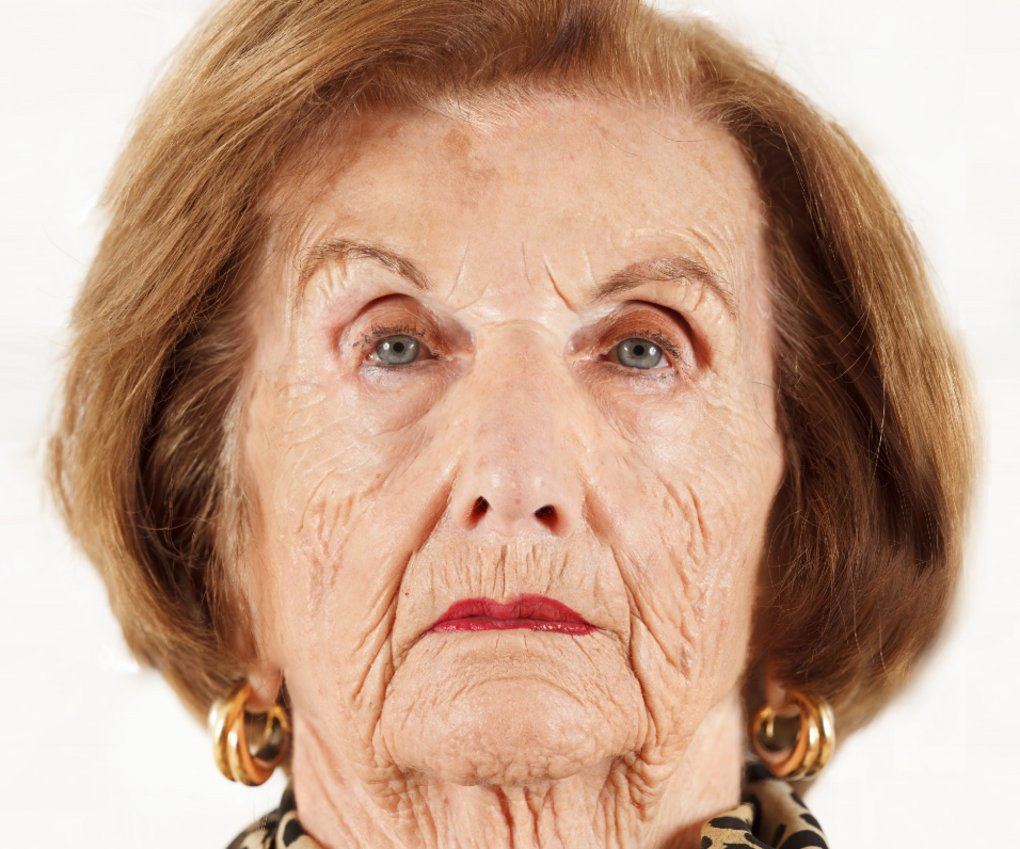
\includegraphics[width=0.95\textwidth]{img/fd3/fail1_input.jpg}
  \caption{}
\end{subfigure}%
\begin{subfigure}{.25\textwidth}
  \centering
  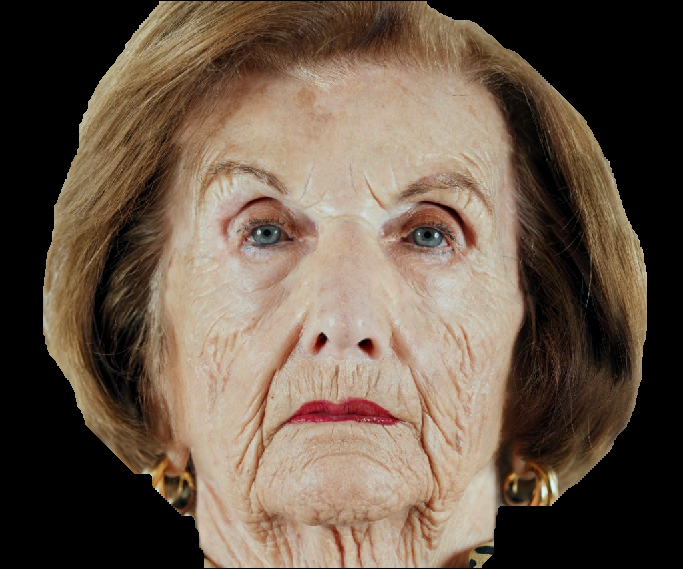
\includegraphics[width=0.95\textwidth]{img/fd3/fail1_faceImage.png}
  \caption{}
\end{subfigure}%
\begin{subfigure}{.25\textwidth}
  \centering
  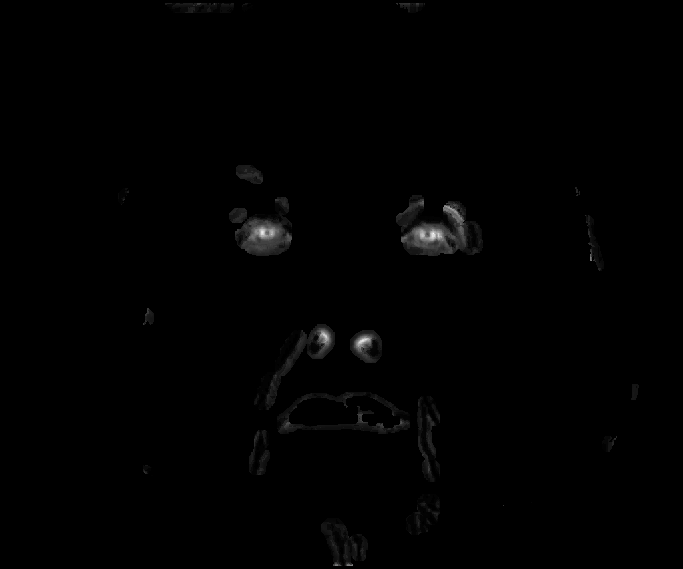
\includegraphics[width=0.95\textwidth]{img/fd3/fail1_finalEyeMap.png}
  \caption{}
\end{subfigure}%
\begin{subfigure}{.25\textwidth}
  \centering
  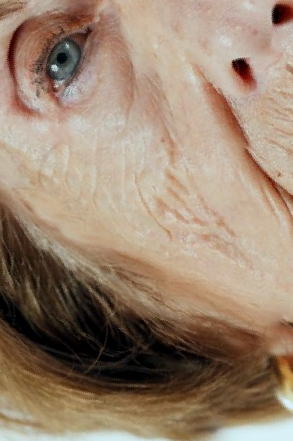
\includegraphics[width=0.53\textwidth]{img/fd3/fail1_output.png}
  \caption{}
\end{subfigure}%

\caption{A case where the proposed algorithm fails to detect the correct face due to an invalid invalid extraction of the eyes from the eye map. (a) show the input image, (b) the correctly extracted face mask, (c) the proper eye map while (d) show the output image where the extraction of the eyes using the Hough transform fail by mixing up the left nostril with the right eye. }
\label{fig:fail1}
\end{figure}


\begin{figure}[H]
\centering

\begin{subfigure}{.25\textwidth}
  \centering
  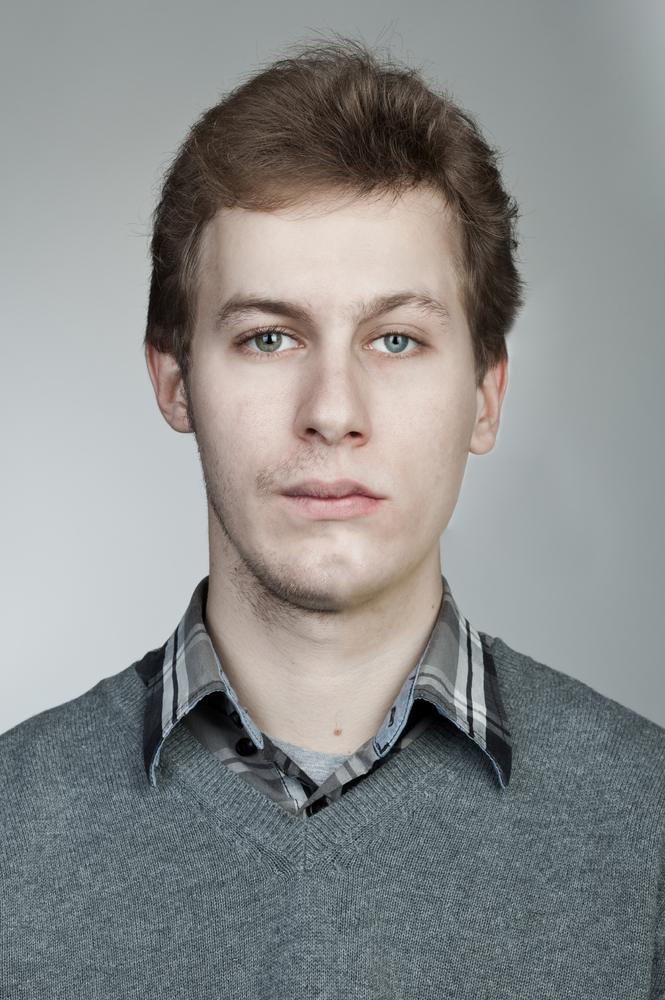
\includegraphics[width=0.53\textwidth]{img/fd3/fail2_input.jpg}
  \caption{}
\end{subfigure}%
\begin{subfigure}{.25\textwidth}
  \centering
  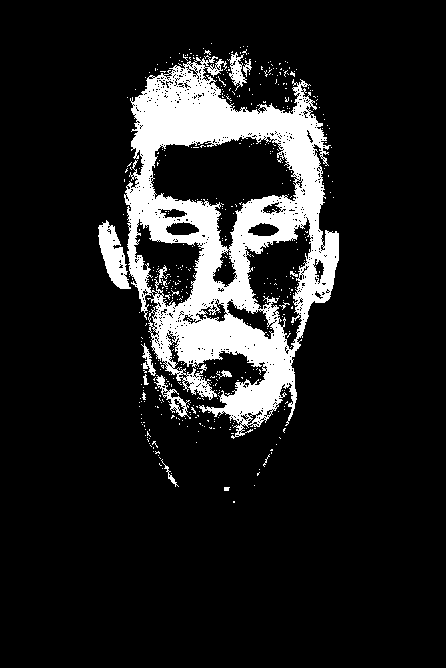
\includegraphics[width=0.53\textwidth]{img/fd3/fail2_estimatedSkinMak.png}
  \caption{}
\end{subfigure}%
\begin{subfigure}{.25\textwidth}
  \centering
  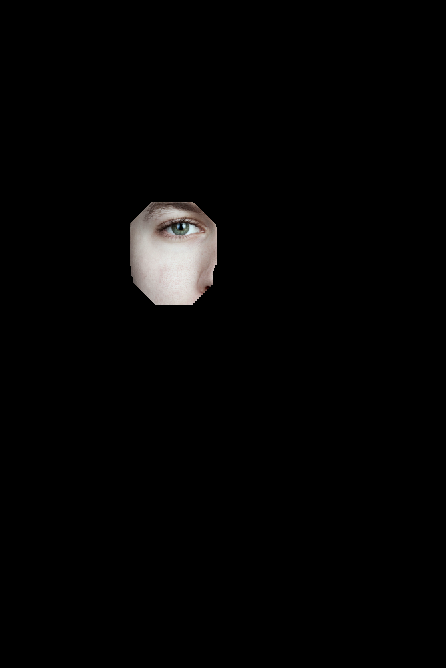
\includegraphics[width=0.53\textwidth]{img/fd3/fail2_faceImage.png}
  \caption{}
\end{subfigure}%
\begin{subfigure}{.25\textwidth}
  \centering
  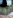
\includegraphics[width=0.23\textwidth]{img/fd3/fail2_output.png}
  \caption{}
\end{subfigure}%

\caption{A case where the proposed algorithm fails to detect the correct face due to a too sparse estimated skin mask. (a) show the input face, (b) the estimated skin mask, (c) the resulting invalid face mask and (d) the output.}
\label{fig:fail2}
\end{figure}




\begin{figure}[H]
\centering

\begin{subfigure}{.25\textwidth}
  \centering
  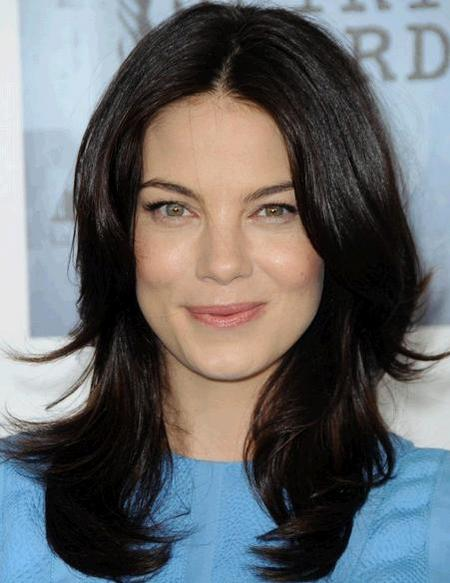
\includegraphics[width=0.53\textwidth]{img/fd3/fail3_input.jpg}
  \caption{}
\end{subfigure}%
\begin{subfigure}{.25\textwidth}
  \centering
  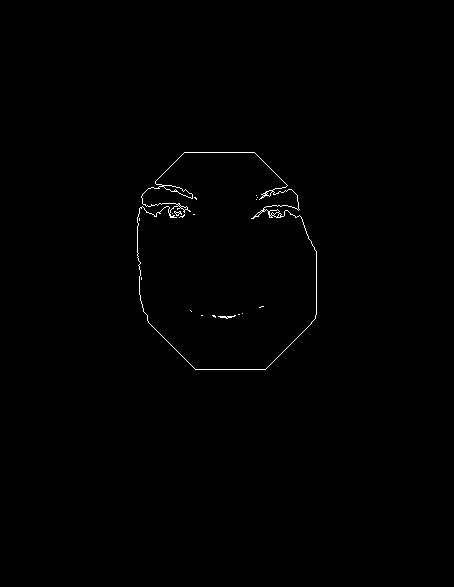
\includegraphics[width=0.53\textwidth]{img/fd3/fail3_faceBorder.png}
  \caption{}
\end{subfigure}%
\begin{subfigure}{.25\textwidth}
  \centering
  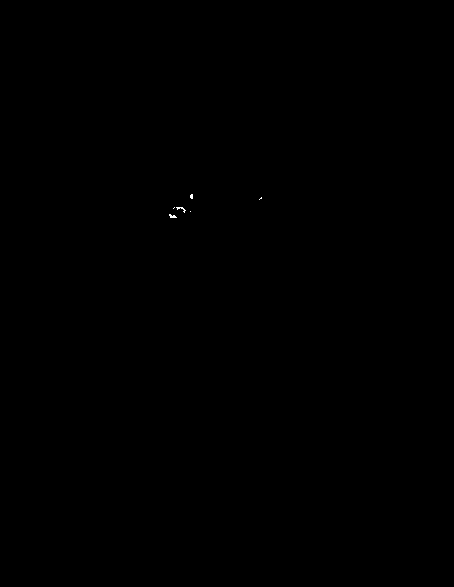
\includegraphics[width=0.53\textwidth]{img/fd3/fail3_eyeCandidates.png}
  \caption{}
\end{subfigure}%
% \begin{subfigure}{.15\textwidth}
%   \centering
%   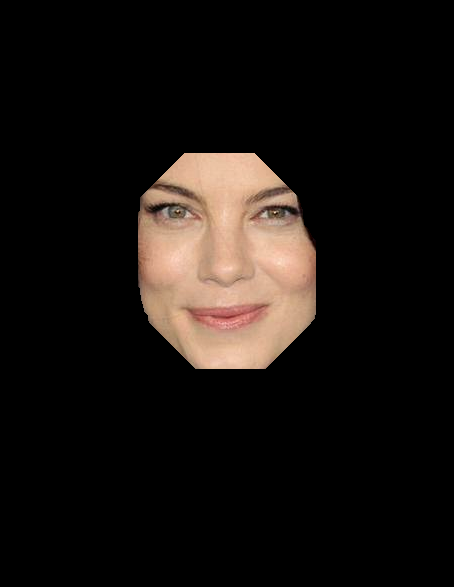
\includegraphics[width=0.53\textwidth]{img/fd3/fail3_faceImage.png}
%   \caption{}
% \end{subfigure}%
% \begin{subfigure}{.15\textwidth}
%   \centering
%   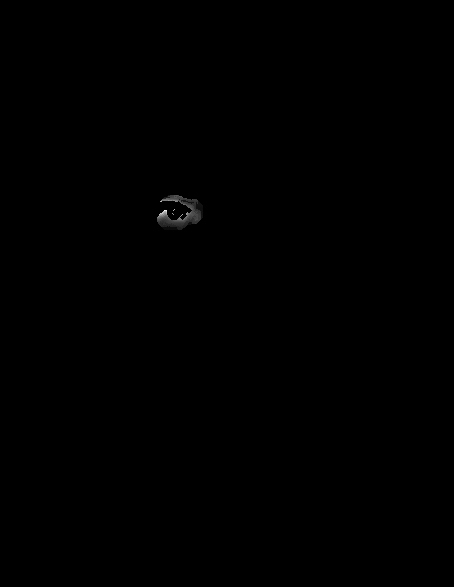
\includegraphics[width=0.53\textwidth]{img/fd3/fail3_finalEyeMap.png}
%   \caption{}
% \end{subfigure}%
\begin{subfigure}{.25\textwidth}
  \centering
  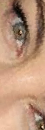
\includegraphics[width=0.23\textwidth]{img/fd3/fail3_output.png}
  \caption{}
\end{subfigure}%

\caption{A case where the proposed algorithm fails to detect the correct face due to a lack of eye candidates for both eyes. (a) show the input image, (b) the filtered face mask that gives the insufficient eye candidates in (c) and lead to the invalid output (d).}
\label{fig:fail3}
\end{figure}




% \begin{figure}[H]
% \centering

% \begin{subfigure}{.25\textwidth}
%   \centering
%   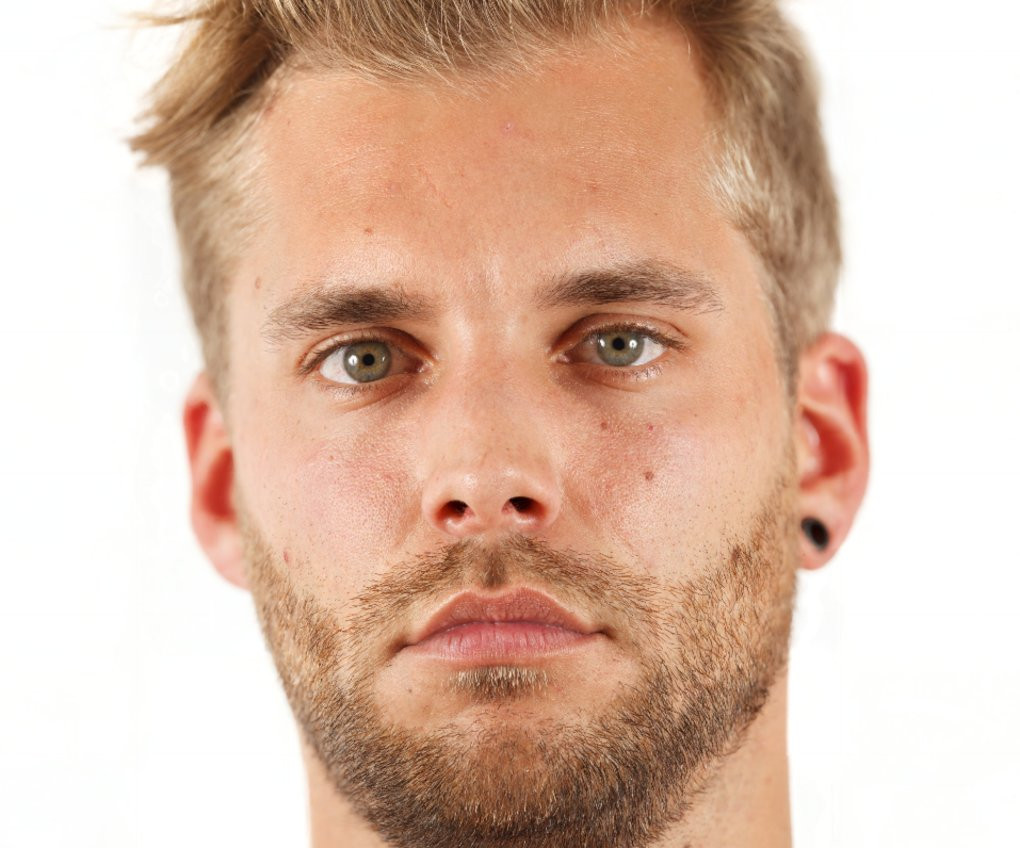
\includegraphics[width=0.95\textwidth]{img/fd3/fail4_input.jpg}
%   \caption{}
% \end{subfigure}%
% \begin{subfigure}{.25\textwidth}
%   \centering
%   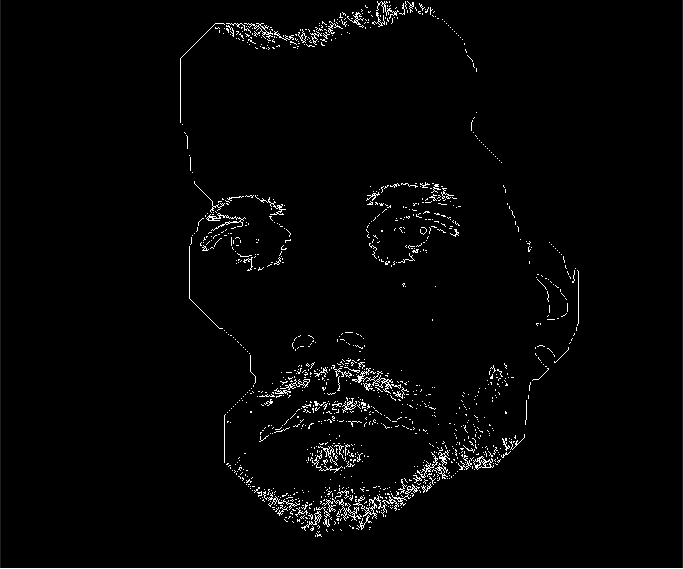
\includegraphics[width=0.95\textwidth]{img/fd3/fail4_faceBorder.png}
%   \caption{}
% \end{subfigure}%
% \begin{subfigure}{.25\textwidth}
%   \centering
%   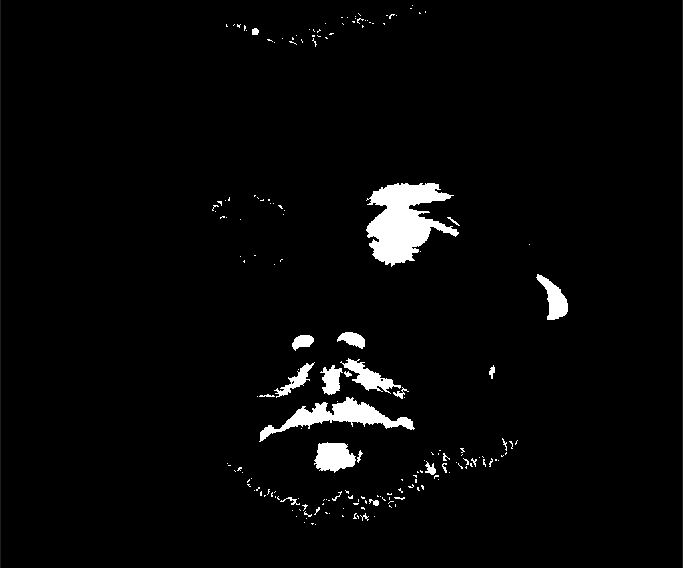
\includegraphics[width=0.95\textwidth]{img/fd3/fail4_eyeCandidates.png}
%   \caption{}
% \end{subfigure}%
% % \begin{subfigure}{.15\textwidth}
% %   \centering
% %   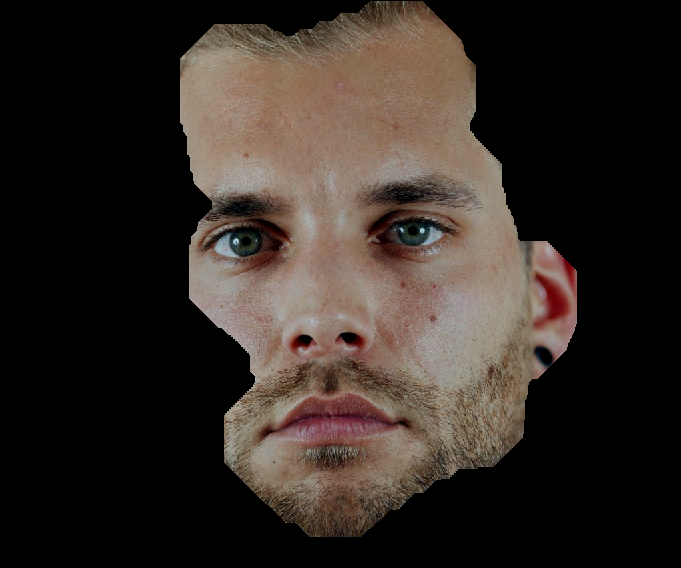
\includegraphics[width=0.95\textwidth]{img/fd3/fail4_faceImage.png}
% %   \caption{}
% % \end{subfigure}%
% % \begin{subfigure}{.15\textwidth}
% %   \centering
% %   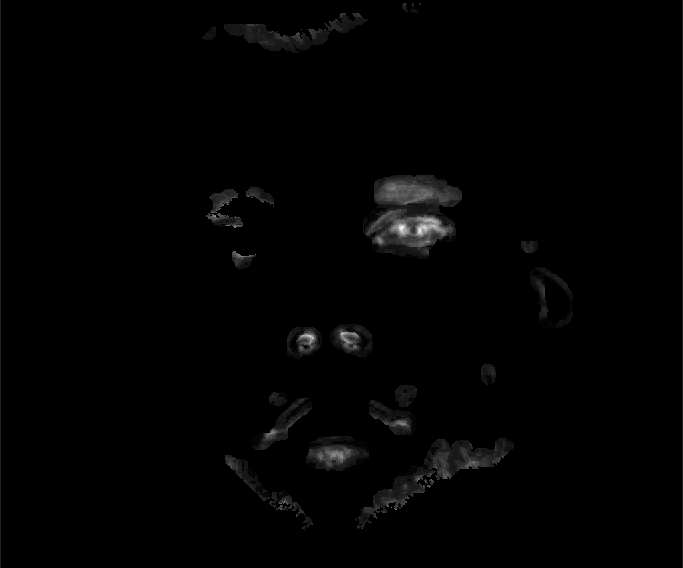
\includegraphics[width=0.95\textwidth]{img/fd3/fail4_finalEyeMap.png}
% %   \caption{}
% % \end{subfigure}%
% \begin{subfigure}{.25\textwidth}
%   \centering
%   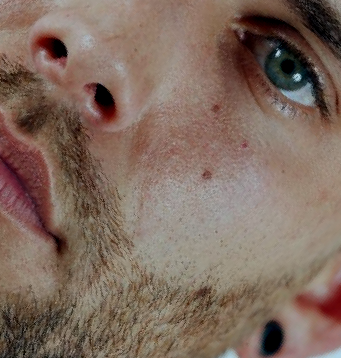
\includegraphics[width=0.53\textwidth]{img/fd3/fail4_output.png}
%   \caption{}
% \end{subfigure}%

% \caption{Resonera, Fail4}
% \label{fig:fail4}
% \end{figure}






